\documentclass[licencjacka]{pracamgr}
\usepackage{amsmath}
\usepackage{graphicx}

\autor{Tomasz Fąs}{382348}


\title{Tunelowanie między studniami kwantowymi umieszczonymi w mikrownęce optycznej.}

\kierunek{Fizyka}


\opiekun{dr hab. Jan Suffczyński\\
  Zakład Fizyki Ciała Stałego\\
  }

\date{Któryś z 2019}

\dziedzina{ 13.2 Fizyka\\ }

%Klasyfikacja tematyczna wedlug AMS (matematyka) lub ACM (informatyka)
\klasyfikacja{Do\\
  ustalenia\\
  chyba}

\keywords{mikrownęka optyczna, tunelowanie, polaryton, ekscyton, fotoluminescencja}

\newtheorem{defi}{Definicja}[section]


\begin{document}

\maketitle

\begin{abstract}
  W niniejszej pracy przedstawiono zależność intensywności tunelowania między studniami kwantowymi od przyłożonego pola magnetycznego. Wykorzystana próbka składała się ze studni kwantowych umieszczonych w mikrownęce. Udało się uzyskać tunelowanie całego ekscytonu tj. elektronu i dziury, przez barierę potencjału o szerokości 125 nm. Doświadczenie to częściowo wypełnia lukę w dziedzinie tunelowania średniodystansowego.
\end{abstract}


\chapter*{Wprowadzenie}
\addcontentsline{toc}{chapter}{Wprowadzenie}
%Miesznie funkcji falowych%
%Ogólny opis, bez wzgłębiania się w szcegóły
%
Jednym z ważniejszych efektów w mechanice kwantowej jest tunelowanie, czyli przejście cząstki z jednej studni potencjału do innej pomimo braku odpowiedniej energii, by przekroczyć barierę między nimi. Prawdopodobieństwo takiego przejścia maleje eksponencjalnie wraz z odległością między studniami. Jednakże prawdopodobieństwo przejścia można zwiększyć korzystając ze sprzężenia między studniami, czyli własności która sprawia, że zmiany stanu jednej ze studni mają wpływ na stan drugiej. W pracy S. A. Gurvitz'a et. al \cite{1991} został przedstawiony taki opis studni sprzężonych wraz ze sposobami na zwiększenie prawdopodobieństwa tunelowania takich jak na przykład manipulacja grubością bariery. Artykuł ten jest oparty na danych eksperymentalnych uzyskanych przez B. Deveaud'a et. al. \cite{1990}, w którym to autorzy badali tunelowanie elektronów na sprzężonych studniach kwantowych o różnej grubości bariery. Udało się im zaobserwować efekt tunelowania przez barierę o grubości 80 \r{A}.  Z kolei I. Lawrence et al. \cite{1994} w pracach nad tunelowaniem wykorzystali ekscyton, czyli parę elektron-dziura, która może powstać np. w półprzewodnikach, kiedy foton wzbudzi elektron z pasma walencyjnego w pobliże pasma przewodnictwa. Taka kwazicząstka jest związane poprzez oddziaływanie kulombowskie i może swobodnie poruszać się w krysztale. Po pewnym czasie dojdzie do jej rekombinacji i emisji fotonu. W swojej pracy autorzy udowodnili, iż możliwe jest tunelowanie takiej cząstki do studni oddalonej o 109 \r{A}. W porównaniu z pracą Deveaud'a   udało się doprowadzić do przetunelowania bardziej złożonego układu na jeszcze większą odległość. %Ekscytony mogą powstawać również w studniach półprzewodnikowych. Jeśli taka para powstanie w tej samej studni, to otrzymamy ekscyton bezpośredni (direct exciton). Jeśli mieliśmy do czynienia z dwiema studniami kwantowymi, a elektron przetunelował do drugiej z nich, to mamy do czynienia z tzw. ekscytonem niebezpośrednim (indirect exciton). Taki ekscyton, rozdzielony barierą potencjału, charakteryzuje się dłuższym czasem życia od ekscytonu bezpośredniego, jak i większym momentem dipolowym. 
Można pójść jeszcze dalej w modyfikowaniu ekscytonu i wprowadzić mikrownękę optyczną, czyli obszar o rozmiarach mikrometrów ograniczony przez zwierciadła. W takiej mikrownęce mogą powstawać elektromagnetyczne fale stojące, czyli mody optyczne. Jeśli w mikrownęce zostanie umieszczona studnia półprzewodnikowa, to uwięziony foton może spowodować powstanie ekscytonu, który następnie zrekombinuje i wyemituje foton. Wyemitowany foton może ponownie doprowadzić do powstania ekscytonu, a cykl się powtórzy. Sprzężenie tego typu, między fotonem a ekscytonem, nazywa się polarytonem. %Wrzucić do fitowania%
 To właśnie na takim sprzężeniu skupiono się w tej pracy. W mikrownęce umieszczono dwie studnie kwantowe: jedna z nich, zwana magnetyczną (MQW) silnie reagowała z polem magnetycznym, co pozwalało na kontrolę jej głębokości. Z kolei druga studnia, zwana niemagnetyczną (NMQW), znacznie słabiej reagowała z polem. Studnie te były otoczone półprzepuszczalnymi zwierciadłami Bragga, umożliwiając wprowadzanie fotonów do wnętrza mikrownęki. Powstałe ekscytony mogły zrekombinować w tej samej studni, w której powstały, lub jako całość przetunelować za pośrednictwem modu optycznego do drugiej z nich i dopiero tam ponownie się połączyć. Badając fotoluminescencję próbki, można określić, czy dochodzi do tunelowania ekscytonów, czy też takowe rekombinują tam, gdzie powstały.

\chapter{Próbka}\label{r:probka}
Próbka została wykonana przez dr hab. Wojciecha Pacuskiego z Zakładu Fizyki Ciała Stałego. Do jej wykonania skorzystano z dwukomorowej maszyny MBE. Całość została wyhodowana na podstawce z (100) GaAs:Si. Dalej zastosowano warstwę buforową CdZnMgTe o grubości 1 $\mu$m. Na buforze wyhodowano 26 par zwierciadeł Bragga oznaczonych jako DBR, 3 studnie kwantowe (Cd,Zn,Mn)Te o grubości 10 nm oddalone od siebie również o 10 nm, barierę z CdZnMgTe o grubości 125 nm i 3 studnie kwantowe CdZnMgTe o grubości 10 nm i odległości od siebie wynoszącej 10 nm. Całość zwieńczają 22 pary zwierciadeł Bragga. Schemat próbki wraz z procentową zawartością pierwiastków znajduje się na Rysunku 1.1.

\begin{figure}[h!]
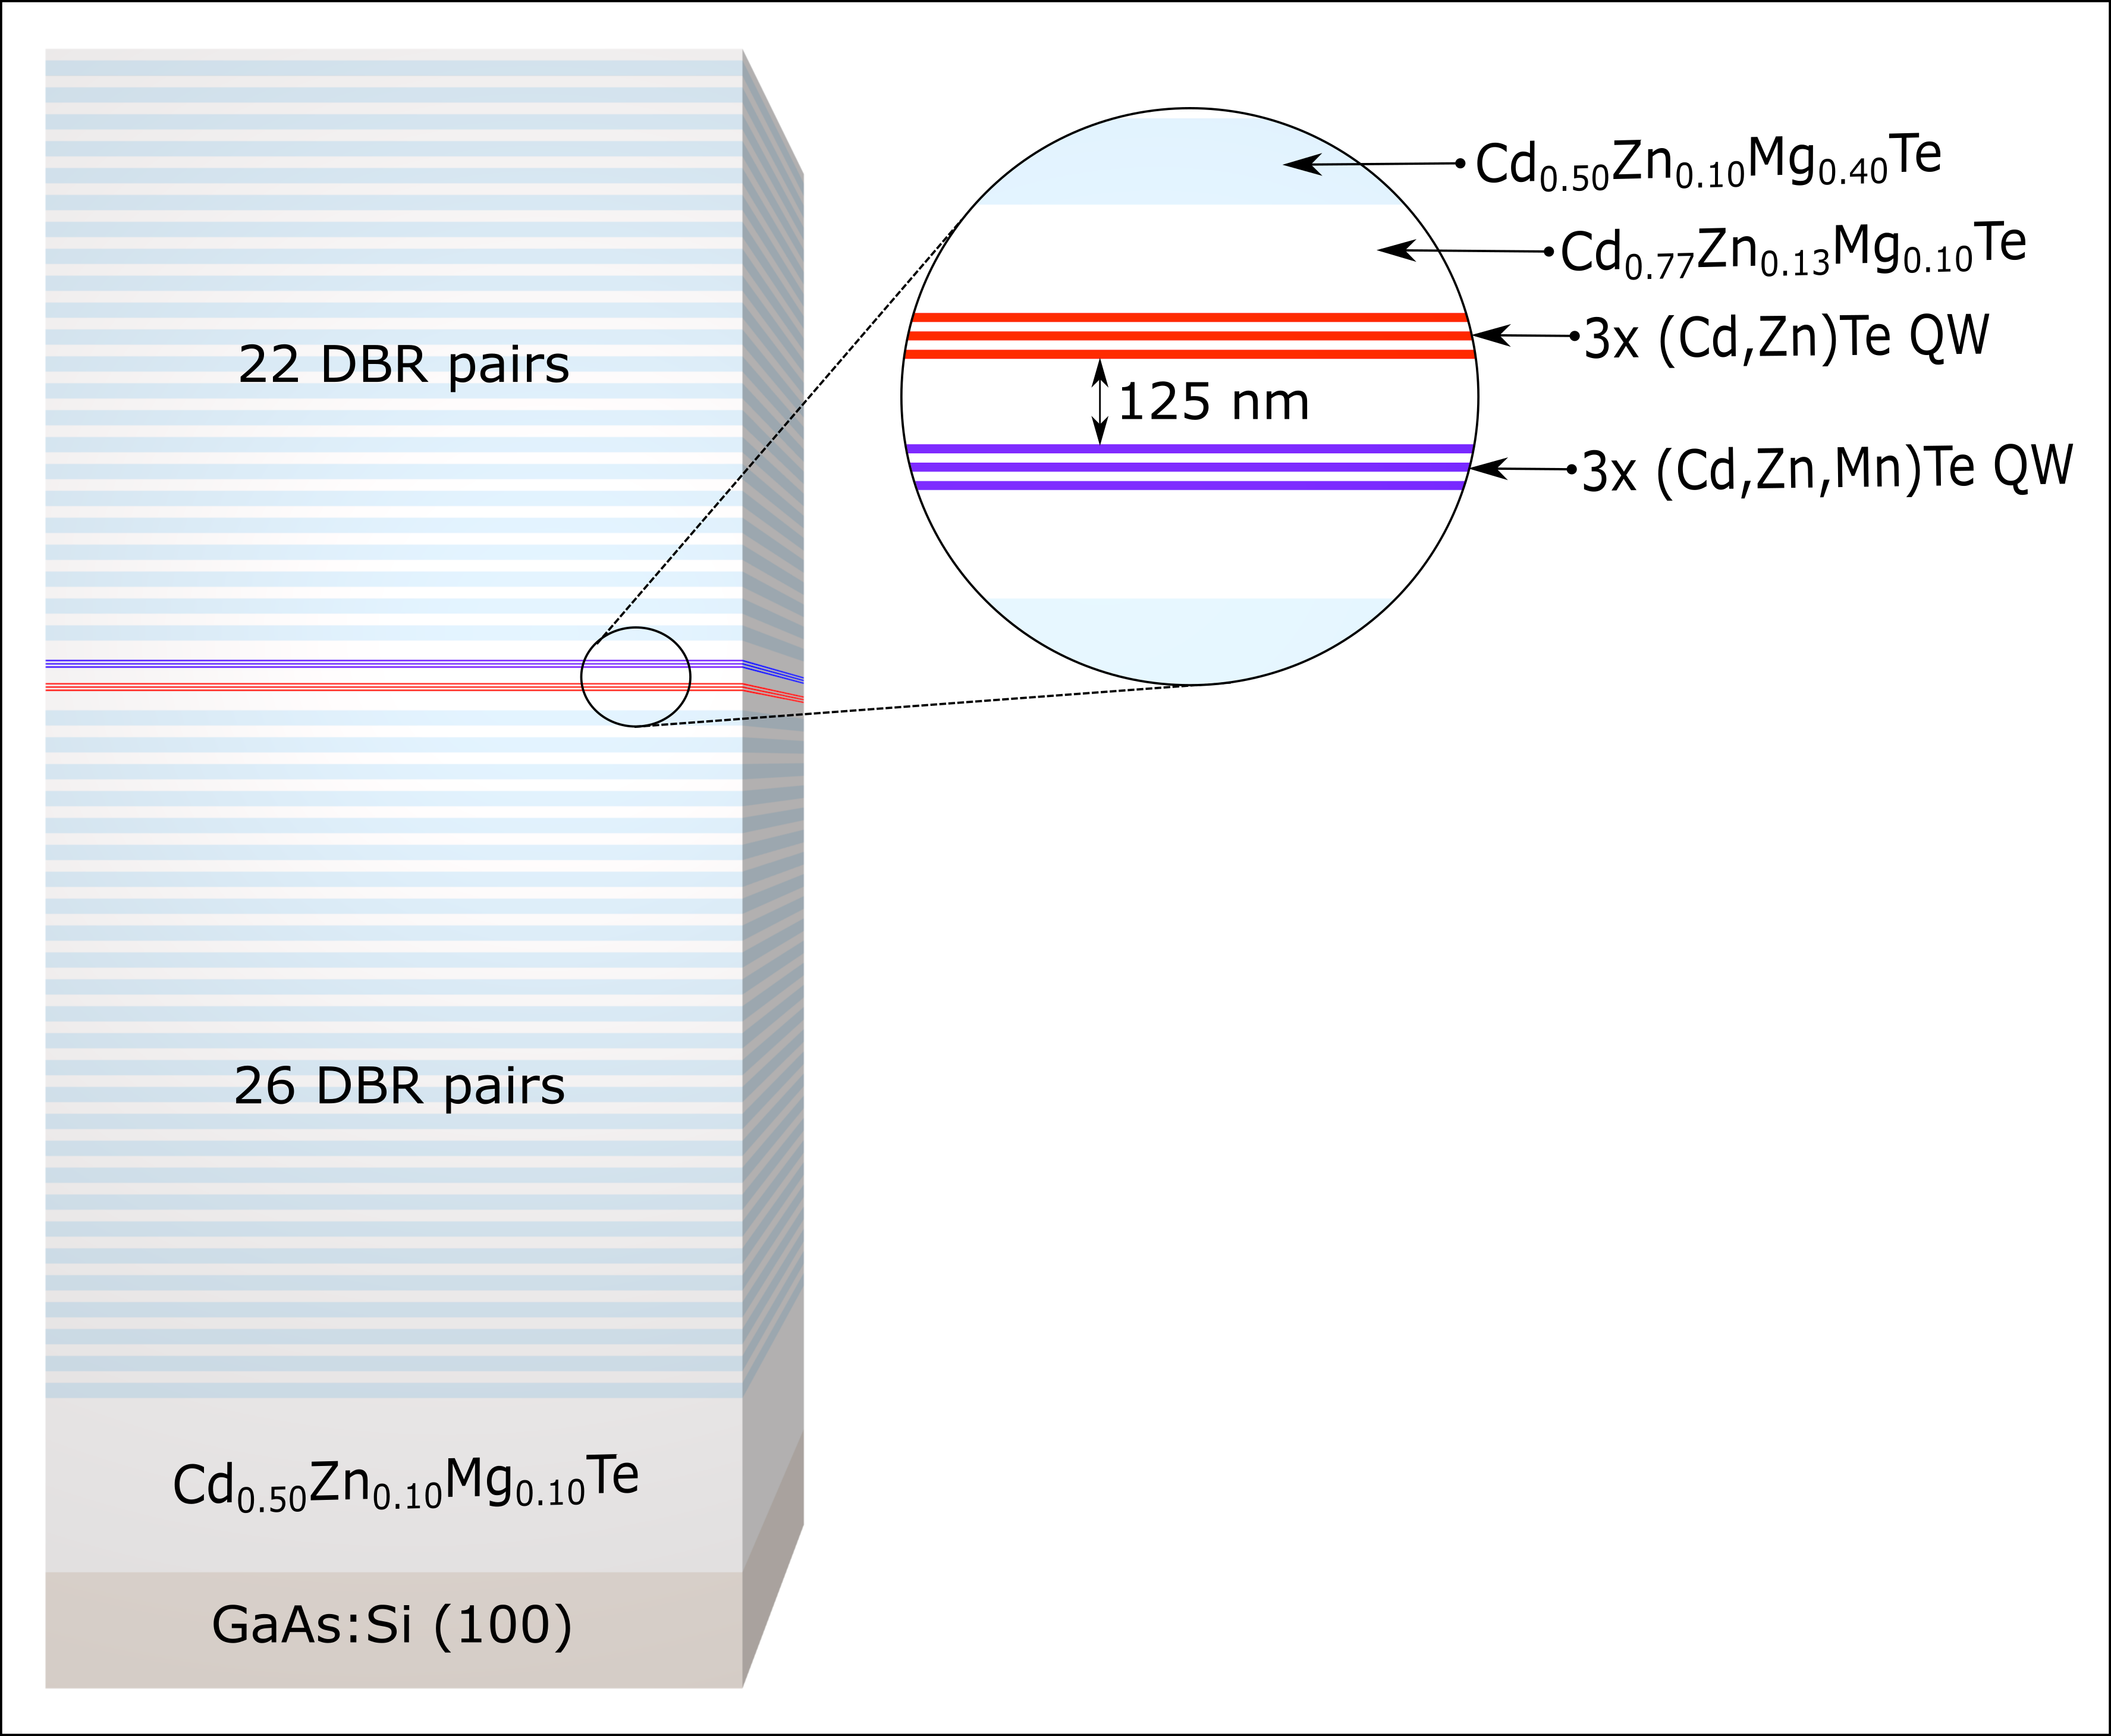
\includegraphics[width=13cm]{Probka.png} 
\centering
\caption{Schemat próbki.}
\end{figure}

Studnie tu wykorzystane są wykonane z materiału typu DMS, czyli półprzewodnika półmagnetycznego. Materiał tego typu wykazuje właściwości zarówno półprzewodnikowe jak i magnetyczne, pozwalając np. na kontrolę jego poziomów energetycznych przy pomocy pola magnetycznego.

\chapter{Metody eksperymentalne}\label{r:metody}
Do wzbudzania ekscytonów wykorzystano laser od długości fali 685 nm, 


\chapter{Wyniki}\label{r:wyniki}

\section{Wyniki surowe}

\section{Dopasowanie do modelu}
 Do opisu próbki można wykorzystać prosty hamiltonian:

\begin{equation}
\hat{H}=
\begin{bmatrix}
\omega_{MQW} & \Omega &0 \\
\Omega & \omega_{C} & \Omega \\
0 & \Omega & \omega_{NMQW}
\end{bmatrix}  
\end{equation}

gdzie $\omega_{MQW}$, $\omega_{NMQW}$ i $\omega_{C}$ oznaczają kolejno energie studni magnetycznej, niemagnetycznej i modu optycznego i są zależne od wartości pola magnetycznego $B$, a $\Omega$ oznacza siłę sprzężenia między studnią a modem.Jak widać, hamiltonian nie opisuje bezpośredniego przejścia z jednej studni do drugiej. Wynika to z szerokiej przerwy między studniami; bezpośredni transport jest pomijalny, jedyny wkład pochodzi od pośrednictwa modu optycznego, czyli procesu postaci rekombinacja $\rightarrow$ powstanie ekscytonu w drugiej studni $\rightarrow$ ponowna rekombinacja w drugiej studni.%



\chapter{Podsumowanie}


\appendix

\chapter{Może będzie potrzebne}

\bibliographystyle{plain}
\bibliography{bibliografia}

\end{document}


%%% Local Variables:
%%% mode: latex
%%% TeX-master: t
%%% coding: latin-2
%%% End:
